\RequirePackage[l2tabu, orthodox]{nag}
\documentclass[11pt, a4paper]{report}

\usepackage[utf8]{inputenc}
\usepackage[a4paper]{geometry}
\usepackage{lmodern}
\usepackage{microtype}
\usepackage{xargs}
\usepackage[pdftex, dvipsnames]{xcolor}
\usepackage[colorinlistoftodos, prependcaption, textsize=tiny]{todonotes}
\usepackage{upquote}
\usepackage{ellipsis}
\usepackage{booktabs}
\usepackage{graphicx} % https://en.wikibooks.org/wiki/LaTeX/Importing_Graphics
\usepackage{dirtree}
\PassOptionsToPackage{hyphens}{url}
\usepackage[colorlinks=false, pdfborder={0 0 0}, unicode=true]{hyperref}
\urlstyle{same} % don't use monospace font for urls

\title{%
    A Perfect Programming Language \\
    \large --- \\
    Version @pom.version@}
\author{Sven Strittmatter}
\date{\today}

\begin{document}

\maketitle

\begin{abstract}
This paper tries to describes what a perfect programming language should constitutes of. We will look at existing programming languages to find what they do well and what are their drawbacks. Then try to describe what such a language must and must not have as features.
\end{abstract}

\tableofcontents

\chapter{Motivation}

What is my motivation behind this: Describe a new perfect programming language? As of time of writing this I have over a decade of experience in programming stuff. I also have experience in various languages: C++, PHP, JavaScript, Ruby, Perl, Java. Also I saw a lot of languages. After some disappointment about the languages I used I started to look around what others do: Go, Python, Erlang, Prolog, Lisp, ML, OCaml, Scala etc.

More and more I saw different languages and their concepts I recognised that most of them have some drawbacks and I started to think about a programming language without any of these. I'm not sure if it is possible to design such a language, but I think it is worth to think about it.

\section{Drawbacks and Fails}

In this section I'll collect all the drawbacks and fails some already existing languages have. These are not drawbacks only because I say. All of them have some common sense in the community of software craftmanship, clean code developers or others working hard on better software. So the points mentioned here are quite common sense for all well exercised developers. In a later section I will describe ``disappointing'' things which are merely based on my opinion.

\subsection{Null --- The Billion Dollar Fail}

In a lot of programming languages exists a concept of \texttt{null}. This is sometimes called a \textit{null reference} or \textit{null pointer}. Most would have seen such a thing somewhere in their career and have a vague idea what it is: Some not initialised value. Let's have a look what Wikipedia\cite{null-wiki} says what it is:

\begin{quotation}
    In computing, a null pointer has a value reserved for indicating that the pointer does not refer to a valid object. Programs routinely use null pointers to represent conditions such as the end of a list of unknown length or the failure to perform some action; this use of null pointers can be compared to nullable types and to the Nothing value in an option type.
\end{quotation}

The first thing to mention here is that different languages implement this concept differently. We do not want to dig to deep into these implementation details but concentrate of the perspective of a user of such languages: The problem then arises is the so called \textit{null dereferencing}. From the same Wikipedia\cite{null-wiki} article:

\begin{quotation}
    Because a null pointer does not point to a meaningful object, an attempt to dereference (i.e.\ access the data stored at that memory location) a null pointer usually (but not always) causes a run-time error or immediate program crash.
\end{quotation}

To repeat the crucial part: ``\ldots causes a run-time error or immediate program crash''. To be clear: the problem is not a concept for a not initialised or not present value, rather than dereferencing such will result in program crashes.

Lets see some brief examples of such null dereferences in various common languages:

\subsubsection{Null in C/C++}
\begin{verbatim}
    SomeType *obj = nullptr;
    obj->methodCall(); // Crashes the program.
\end{verbatim}

\subsubsection{Null in Java}
\begin{verbatim}
    SomeType obj = null;
    name.methodCall(); // Crashes the program.
\end{verbatim}

\subsubsection{Null in C\#}
\begin{verbatim}
    SomeType obj = null;
    obj.MethodCall(); // Crashes the program.
\end{verbatim}

\subsubsection{Null in JavaScript}
In JavaScript there is also \textit{undefined}. It is slightly different than null, but this does not matter for the fact that \textit{null dereferences} crashes. Maybe this undefined thing is as bad as null too.

\begin{verbatim}
    var obj = null;
    obj.methodCall(); // Crashes the program.

    obj = {methodCall: null};
    obj.methodCall(); // Crashes the program.
\end{verbatim}

\subsubsection{Null in PHP}
\begin{verbatim}
    $obj = null;
    obj->methodCall(); // Crashes the program.
\end{verbatim}

\subsubsection{None in Python}
\begin{verbatim}
    obj = None
    obj.methodCall() # Crashes the program.
\end{verbatim}

\subsubsection{Nil in Ruby}
\begin{verbatim}
    obj = nil
    obj.method_call # Crashes the program.
\end{verbatim}

\subsubsection{Null in Perl}
\begin{verbatim}
    my $obj;
    $obj->method_call; # Crashes the program.
\end{verbatim}

All these examples above will compile/translate without any error, but will crash tremendously at runtime. Some might say this is not a problem rather than the concept of the particular language and as a developer you have to deal with such issues: you have to write your program either that you do not produce such null values or you deal with them correctly. But this is easier said than done. To paraphrase Murphy's law\cite{murphys-law}: If there is the possibility to make something wrong, then someone will do it wrong at some point in time. So as a result developers tend to clutter up code with null checks (called defensive programming). Which will make the code harder to read and reason. As Kent\cite{kent-dyn-err-remediation} stated in his paper \textit{Dynamic Error Remediation: A Case Study with Null Pointer Exceptions}:

\begin{quotation}
    One insidious bug is the null pointer exception, which by its ``null'' nature is hard for programmers to fix. These bugs indicate that nothing was found in memory where something should have been, giving programmers very little to work with to fix the bug besides a stack trace. Null pointer exceptions sometimes show themselves only with certain inputs, making these bugs difficult to find before deployment. \ldots, 1--2\% of developer code is devoted to identifying null objects.
\end{quotation}

Also an important argument is the economic damage done by this kind of bugs. Kent\cite{kent-dyn-err-remediation} cites the NIST that along with developer time and money spent in error checking annually cost of \$59.5 are estimated. From the origin source it is not clear that these costs only came from this kind of bug or from all kinds. Anyway what the real numbers are (it is always difficult to estimate such numbers reliably), the sheer amount mentioned in that paper gives a hint of the the caused damage. This is the same what Tony Hoare\cite{hoare-wiki} the inventor of \textit{null} said later it\cite{hoeare-null} in retrospection:

\begin{quotation}
    I call it my billion-dollar mistake. It was the invention of the null reference in 1965. At that time, I was designing the first comprehensive type system for references in an object oriented language (ALGOL W). My goal was to ensure that all use of references should be absolutely safe, with checking performed automatically by the compiler. But I couldn't resist the temptation to put in a null reference, simply because it was so easy to implement. This has led to innumerable errors, vulnerabilities, and system crashes, which have probably caused a billion dollars of pain and damage in the last forty years.	
\end{quotation} 

Whatever the real economic damage is, the fact that this kind of bug is completely avoidable by removing null pointers is obvious. To be clear: There is no problem with the concept that a value may or may not be present. Some languages (as described later) has implemented this without null pointers. The problem with null pointers is that everything everywhere may be one and either you put lot of checking code into your software or you risk crashes. In statically typed language this also subverts the type system because every type may be null but the statically checking at compile time can't inform you about this problem. As mentioned above the problem will hit reality first at runtime. There are lot of more problems which will be introduced by null. A list of some is described by Paul Draper in his blog post \textit{The worst mistake of computer science}\cite{draper-worst-mistake-cs}.

Of course there are techniques to circumvent null pointer dereferences in such languages without cluttering up the code with lot of null checks and boiler plate code. You can avoid using null at all. Use empty strings or zero instead of null. Or use \textit{Null Object Pattern} is a special kind of object of your type which represent an absent value. But these are workarounds and introduce the big caveat that a software developer need to know about. Remember yourself starting software development as a novice: You learned about that null thing in your language of choice and of course you used it. Why else should it be part of the language, unless to use it?

Now the interesting question is: \textit{How to deal with values which may or may not be present without introducing null pointers?} Let's look at some languages which try this:

\subsubsection{Nil in Objective-C}
Despite the fact that \textit{Objective-C} has null due to its inheritance from C (because it is build on top of C). It has an interesting concept called \textit{nil}. It is nearly the same as the C null (instead of \texttt{(void *)0} it is \texttt{(id)0}). The big difference is that you can send method calls to \textit{nil} without getting an error. The call is simply ignored and returns \textit{nil} as result. So consecutive calls will not fail. This obviates defensive programming as mentioned above. For example a if-expression like

\begin{verbatim}
    if (name != nil && [name isEqualToString:@"Hello, World!"]) {
        ...
    }
\end{verbatim}

\noindent can be simplified to

\begin{verbatim}
    if ([name isEqualToString:@"Hello, World!"]) { 
        ...
    }
\end{verbatim}

\noindent So it is an \textit{opt-in procedure} to ask if a value is \texttt{nil}: In the special case you do not want it you can react on it, but by default the program does not crash. But \textit{Objective-C} has some drawbacks in the field of not initialised references: First it has the C null as mentioned above. This introduces the risk that it is used (if someone didn't know better). Second it is not possible to store \texttt{nil} in collection types and so there is a special container type singleton for that: \texttt{NSNull}. Also there is a distinction between uninitialised object references (\texttt{nil}) and uninitialised class references (\texttt{Nil}). This makes the whole thing complicated and error prone if someone is not familiar with the whole concept.

\subsubsection{Nil in Go}
Go has the philosophy that \textit{value types} should be preferred to pointer types. So a value type will never be \texttt{nil} (which is the Go equivalent for \texttt{null}), but a value which has all its properties set to a zero value\cite{golang-spec}. So this example will never fail

\begin{verbatim}
    var t time.Time
    t.Day()
\end{verbatim}

But there are no checks if this is done intentionally or if the developer only forgot to call a constructor function. But it will not crash the application because the variable \texttt{t} will be properly initialised to a zeroed value. That mean all primitive values such as numbers, booleans, character sequences, collections etc./ are set to an zero equivalent value. Because of the fact that all complex data structures are made of these primitives it is possible to create zeroed values transitively. But it is possible to have an equivalent to a \textit{null pointer dereference}:

\begin{verbatim}
    var t *time.Timer = nil
    t.Reset(10) // Crashes the program.
\end{verbatim}

\subsubsection{Nil in Swift}

Nil in Swift is quite similar to Nil in Objective-C:\@

\begin{quotation}
    Optional chaining in Swift is similar to messaging nil in Objective-C, but in a way that works for any type, and that can be checked for success or failure.\cite{swift-spec-optional-chaining}
\end{quotation}

This is done by adding a special operator \texttt{?} for the so called \textit{Optional Chaining}, e.g.

\begin{verbatim}
    john.residence?.numberOfRooms
\end{verbatim}

This will not fail if \texttt{residence} is \textit{nil}. But it introduces the drawback named \textit{Forced Unwrapping}. If the above example is changed to

\begin{verbatim}
    john.residence!.numberOfRooms
\end{verbatim}

and \texttt{residence} is \textit{nil} then the program crashes due to a so called \textit{Forced Unwrapping} of \textit{nil}:

\begin{quotation}
    The main difference is that optional chaining fails gracefully when the optional is nil, whereas forced unwrapping triggers a runtime error when the optional is nil.\cite{swift-spec-optional-chaining}
\end{quotation}

\subsubsection{Null in F\#}

F\# is a functional language and does not use \textit{null}. This means there is a \textit{null}, but it should not be used. Only for special circumstances:

\begin{quotation}
    The null value is not normally used in F\# for values or variables. However, null appears as an abnormal value in certain situations. If a type is defined in F\#, null is not permitted as a regular value unless the AllowNullLiteral attribute is applied to the type. If a type is defined in some other .NET language, null is a possible value, and when you are interoperating with such types, your F\# code might encounter null values.\cite{null-in-fsharp}
\end{quotation}

\noindent
So by default F\# uses the concept of optionals\cite{optional-in-fsharp}. A simple example:

\begin{verbatim}
    let keepIfPositive (a : int) = 
        if a > 0 
        then Some(a) 
        else None
\end{verbatim}

\noindent And checking the presence is done with pattern matching:

\begin{verbatim}
    let exists (x : int option) =
        match x with
        | Some(x) -> true
        | None -> false
\end{verbatim}

The downside is that \textit{null} may be present due to the fact that in F\# any other .NET language code can be imported. So you can use C\# code in your F\#. C\# does have \textit{null} and so F\# must deal with that. This drawback is enforced by the .NET ecosystem in which you can mix the different languages.

\subsubsection{Conclusion}

In general there seems to be nothing wrong to have a concept for representing a \textit{not present value} in a programming language. But as shown above most implementations do this in a problematic way which make it far to easy to introduce bugs in production and will cause an application crash.

I'm not sure which concept is better: Add a \textit{Maybe Type} to the language (like F\# and many other functional languages does) or a \textit{nil} with \textit{Optional Chaining} (like Objective-C or Swift). Anyway which one or a combination would be the best, or any other concept I didn't get yet. There is one major problem all of them have: If you can introduce third party components which have a classical \textit{null}, then this will leak into your component. For example in your language it is possible to link good old C libraries (a lot of languages allow such), then you have to deal with possible \textit{null pointers} (Figure ~\ref{fig:Null_from_linked_native_libs}). 

\begin{figure}[ht]
    \centering
    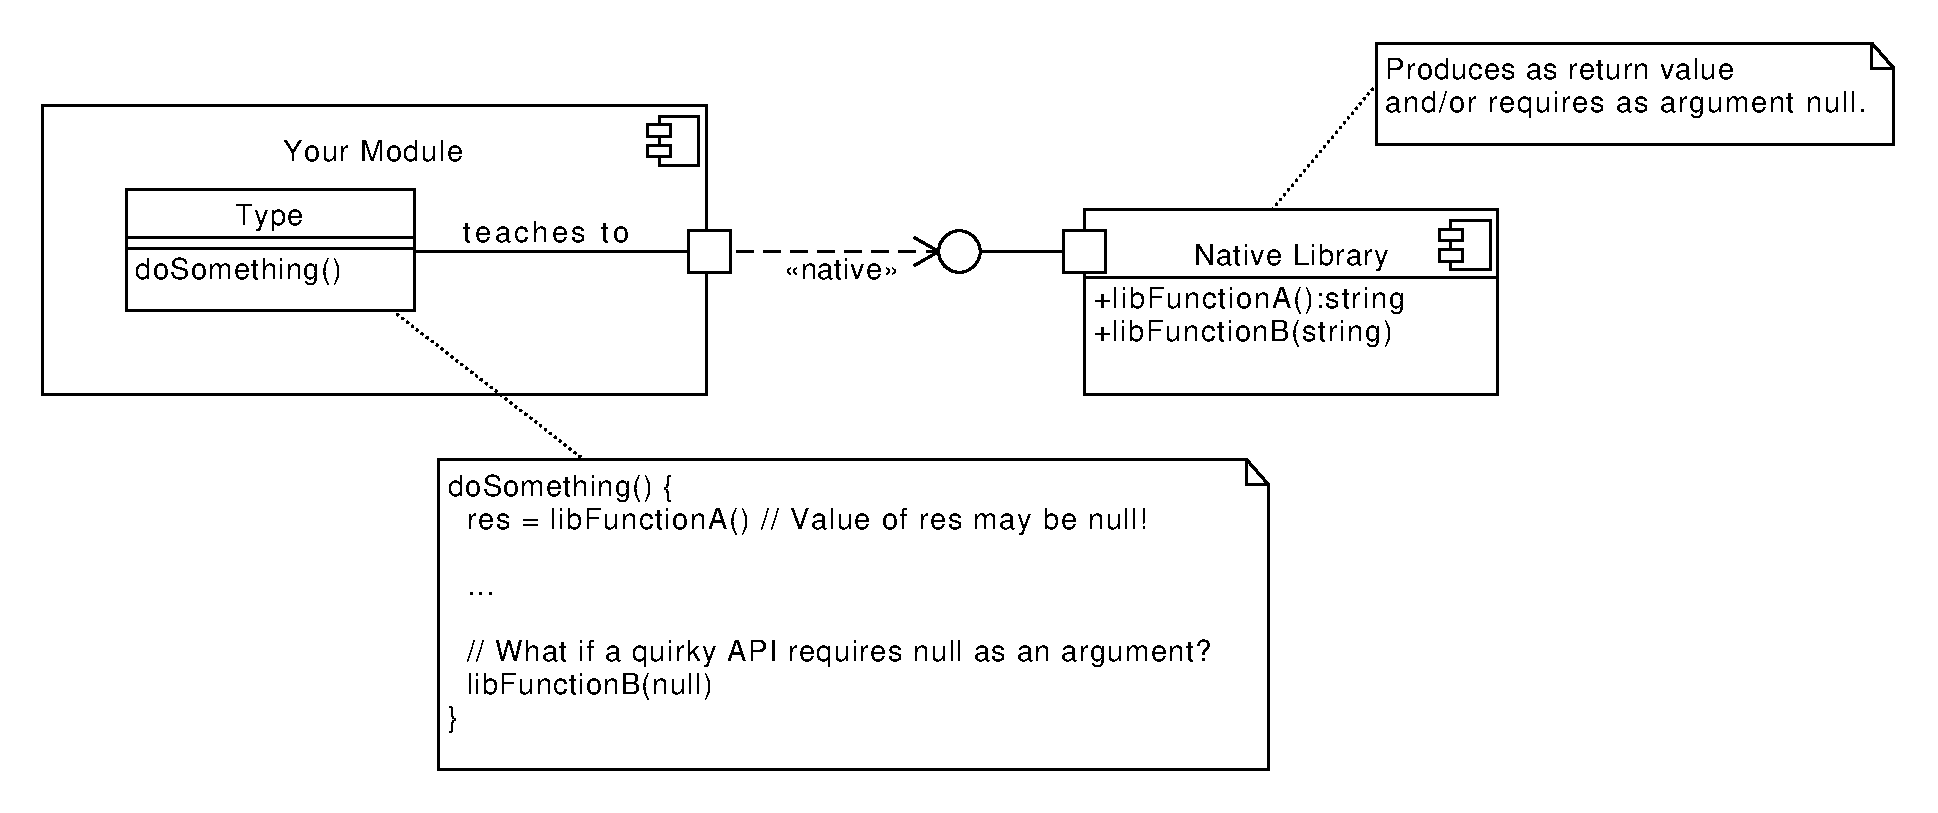
\includegraphics[width=350pt]{grafics/Null_from_linked_native_libs.pdf}
    \caption{Null from a linked native library (e.g.\ a C library)}
    \label{fig:Null_from_linked_native_libs}
\end{figure}

That's the reason why F\#, Objective-C and Swift have something like \textit{null} at certain places. In the F\# documentation they recommend to minimise the use of this ``null'' only at a small place in your code, e.g.\ in a wrapper which delegates to the other library and deals with the \textit{null}. You always need such a layer to maintain type conversions. Some languages gives you more or less help to generate this boiler plate code to bind a native third party library. In my opinions such tooling must be part of the official language specification and implementation. Then you can simply automate the dealing with \textit{null} under the hood and completely transparently (Figure
 ~\ref{fig:Generated_wrapper_for_linked_native_libs}).

\begin{figure}[ht]
    \centering
    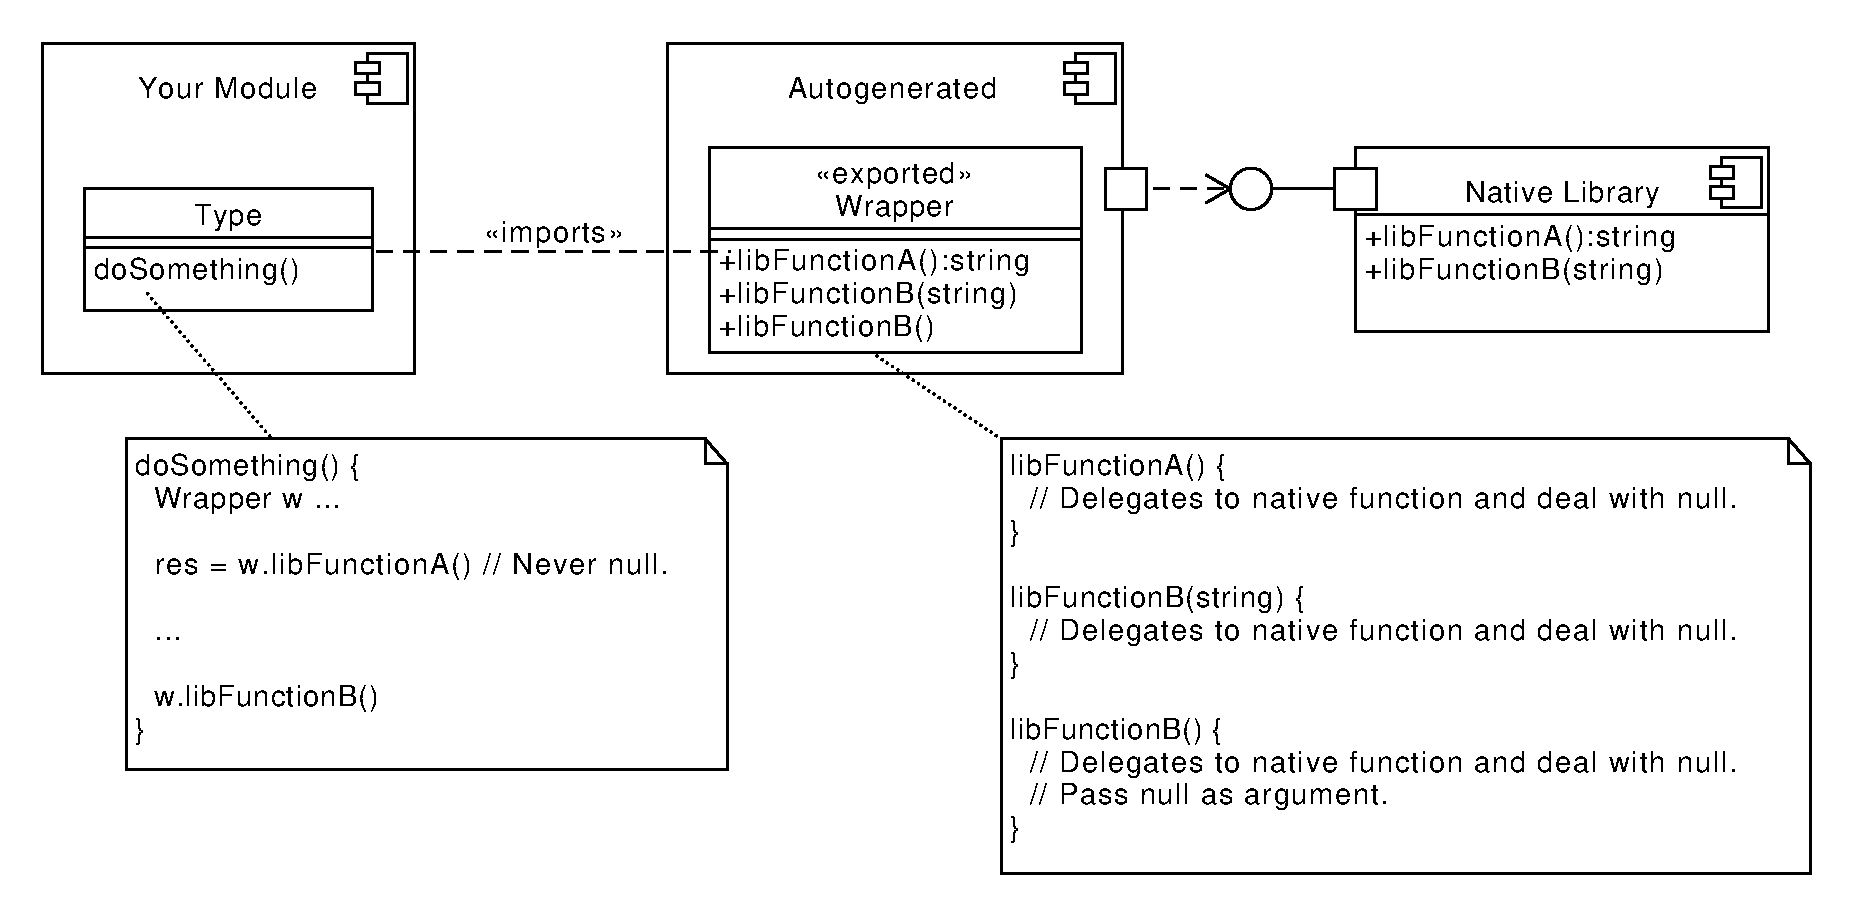
\includegraphics[width=350pt]{grafics/Generated_wrapper_for_linked_native_libs.pdf}
    \caption{Auto generated wrapper which deals with \textit{null} from linked native library (e.g.\ a C library)}
    \label{fig:Generated_wrapper_for_linked_native_libs}
\end{figure}

\subsection{Checked Exceptions}

\todo{Words from Andre Heilsberg (C\#)}

\subsection{Exceptions at All}

\todo{They are like goto (Javaslang)}

\subsection{Compiler Warnings}

\todo{Why are they there? Either it is correct for the compiler or not!}

\section{Disappointing}

In this section I describe things which are very disappointing, e.g.\ typing boiler plate code, parens, semicolons and such. In contrast to the section before these points are merely opinion based. But I try to show why we should think about it.

\subsection{Annoying Braces}

\todo{Braces for conditions: if (condition) vs.\ if condition.}

\subsection{Unnecessary Semicolon}

\todo{Write text for unnecessary semicolons}

\subsection{Too Many Special Character Methods or Operators}

Looking at Perl or Scala as a beginner you will notice a lot of strange characters in the code. Some examples from Perl\cite{secret-perl-operators}:

\begin{itemize}
    \item Spaceship operator: \texttt{<=>}
    \item Eskimo Greeting operator: \texttt{}{}
    \item Goatse operator: \texttt{=()=}
    \item Turtle operator: \texttt{@{[]}}
    \item Inchworm operator: \texttt{~~}
    \item Inchworm-On-A-Stick Operator: \texttt{~-}
    \item Spacestation Operator: \texttt{-+-}
    \item Venus operator: \texttt{0+}
\end{itemize}

Perl is an ancient language, but modern languages also have this problem. Here some examples from Scala\cite{special-operators-scala}:

\begin{itemize}
    \item Upper, lower and view bounds: \texttt{<: >: <\%}
    \item Vararg expansion: \texttt{\_*|}
    \item Many different meanings: \texttt{\_}
\end{itemize}

I don't want to blame Perl or Scala in particular here. Other languages does this also: Haskell, Ruby etc. Especially functional languages tend to strange characters to name functions, methods or operators. In my opinion this violates the rule that source code should be least astonishing. Of course for a professional developer this may be time saving to type three characters instead of a long function name. This argument counted decades ago when the developers only had dumb text editors. Today we all have super power driven editors or IDEs with intellisense and auto completion. So there is no reason to confuse developers without years of experience with strange characters.

\subsection{Missing Tools}

A lot of languages lack of appropriate tooling and it is necessary to build them first before you get productive. A perfect language must come with all necessary tools. What are necessary tools?

All languages have at least a compiler or interpreter. And mostly that's all you get. In my opinion there must be more tools for:

\begin{itemize}
    \item source code formatting
    \item create API docs and documentation
    \item run tests with coverage reports
    \item dependency management
\end{itemize}

\chapter{What Ideas Are Out There?}

In this section interesting ideas and concepts of already existing languages will be described.

\section{Kotlin}

From a blog post from Peter Sommerhoff\cite{kotlin-sommerhoff}:

\subsection{Data Classes}

Simple POJOs are declared simpler. Instead of writing boiler plate like:

\begin{verbatim}
class Book {
    private String title;
    private Author author;

    public String getTitle() {
        return title;
    }
    
    public void setTitle(String title) {
        this.title = title;
    }

    public Author getAuthor() {
        return author;
    }
    
    public void setAuthor(Author author) {
        this.author = author;
    }
}
\end{verbatim}

You can write:

\begin{verbatim}
data class Book(var title: String, var author: Author) {
    // ...
}
\end{verbatim}

\subsection{Smart Casts}

Instead of:

\begin{verbatim}
if (node instanceof Leaf) {
    return ((Leaf) node).symbol;
}
\end{verbatim}

less verbose:

\begin{verbatim}
if (node is Leaf) {
    return node.symbol;
}
\end{verbatim}

\subsection{Type Inference}
\todo{Write text for type inference.}

\subsection{Functional Programming}
\todo{Write text for functional programming.}

\subsection{Default Arguments}
\todo{Write text for default arguments.}

\subsection{Named Arguments}
\todo{Write text for named assignments.}

\subsection{Final Classes}

\begin{quotation}
Next, Kotlin also supports the principle to either design for inheritance or prohibit it — because in Kotlin, you have to explicitly declare a class as open in order to inherit from it. That way, you have to remember to allow inheritance instead of having to remember to disallow it.\cite{kotlin-sommerhoff}
\end{quotation}

\listoffigures

\begin{thebibliography}{100}
	
\bibitem{null-wiki}
    Wikipedia,
    \emph{Null pointer},
    \url{https://en.wikipedia.org/wiki/Null_pointer}

\bibitem{kent-dyn-err-remediation}
    Stephen W. Kent,
    \textit{Dynamic Error Remediation: A Case Study with Null Pointer Exceptions},
    \url{http://citeseerx.ist.psu.edu/viewdoc/download?doi=10.1.1.140.2544&rep=rep1&type=pdf}

\bibitem{hoare-wiki}
    Wikipedia,
    \textit{Tony Hoare},
    \url{https://en.wikipedia.org/wiki/Tony_Hoare}
    
\bibitem{hoeare-null}
    Tony Hoare,
    \textit{Speaking at a conference in 2009},
    \url{http://www.infoq.com/presentations/Null-References-The-Billion-Dollar-Mistake-Tony-Hoare}

\bibitem{draper-worst-mistake-cs}
    Paul Draper,
    \textit{The worst mistake of computer science},
    \url{https://www.lucidchart.com/techblog/2015/08/31/the-worst-mistake-of-computer-science/}

\bibitem{kotlin-sommerhoff}
 	Peter Sommerhoff,
 	\textit{Kotlin for Java Developers: 10 Features You Will Love About Kotlin},
 	\url{https://www.javacodegeeks.com/2016/05/kotlin-java-developers-10-features-will-love-kotlin.html}

\bibitem{secret-perl-operators}
    Peteris Krumin,
    \textit{Secret Perl Operators},
    \url{http://www.catonmat.net/blog/secret-perl-operators/}

\bibitem{special-operators-scala}
    Daniel C. Sobral,
    \textit{What do all of Scala's symbolic operators mean?},
    \url{http://stackoverflow.com/questions/7888944/what-do-all-of-scalas-symbolic-operators-mean}
    
\bibitem{murphys-law}
    Wikipedia,
    \textit{Murphy's law},
    \url{https://en.wikipedia.org/wiki/Murphy's_law}

\bibitem{golang-spec}
    Go Programming Language,
    \textit{The Go Programming Language Specification},
    \url{https://golang.org/ref/spec}

\bibitem{swift-spec-optional-chaining}
    The Swift Programming Language,
    \textit{Optional Chaining},
    \url{https://developer.apple.com/library/content/documentation/Swift/Conceptual/Swift_Programming_Language/OptionalChaining.html}
    
\bibitem{null-in-fsharp}
    F\# Language Reference,
    \textit{This topic describes how the null value is used in F\#},
    \url{https://docs.microsoft.com/en-us/dotnet/articles/fsharp/language-reference/values/null-values}.

\bibitem{optional-in-fsharp}
    F\# Language Reference,
    \textit{Options},
    \url{https://docs.microsoft.com/en-us/dotnet/articles/fsharp/language-reference/options}

\end{thebibliography}

\end{document}
